\documentclass[aspectratio=169, 10pt]{beamer}
\usetheme{metropolis}
% \usefonttheme{professionalfonts}

\usepackage[english]{babel}
\usepackage[style=authortitle,backend=biber]{biblatex}
\usepackage[utf8]{inputenc}
\usepackage{algorithmic}
\usepackage{amsfonts}
\usepackage{amsmath}
\usepackage{amssymb}
\usepackage{array}
\usepackage{booktabs}
\usepackage{caption}
\usepackage{colortbl}
\usepackage{csquotes}
\usepackage{graphicx}
\usepackage{heuristica}
\usepackage{hyperref}
\usepackage{mathptmx}
\usepackage{multirow}
\usepackage{pgfplots}
\usepackage{siunitx}
\usepackage{subcaption}
\usepackage{svg}
\usepackage{tabularx}
\usepackage{textcomp}
\usepackage{xcolor}
\usepackage{bm}
% \usepackage{minted}

\addbibresource{references.bib}

\usetikzlibrary{calc}

% \pgfplotsset{compat=1.17}
\usepgfplotslibrary{statistics}

\definecolor{uniblue}{HTML}{00467f}
\definecolor{uniblueDark}{HTML}{002052}
\definecolor{uniblueLight}{HTML}{4671af}
\definecolor{blueGrey}{HTML}{cfd8dc}
\definecolor{red800Dark}{HTML}{8e0000}
\definecolor{green800Dark}{HTML}{005005}

\setbeamercolor{background canvas}{bg=white}
% \setbeamertemplate{frame footer}{\insertshortauthor}
\setbeamerfont{page number in head/foot}{size=\tiny}
% \setbeamercolor{footline}{fg=white, bg=uniblue}
\setbeamercolor{footline}{fg=uniblue}
\setbeamercolor{title}{fg=uniblueDark, bg=white}
\setbeamercolor{frametitle}{fg=white, bg=uniblue}
\setbeamercolor{progress bar}{fg=uniblueLight, bg=white}
\setbeamercolor{block title}{use=structure,fg=white,bg=uniblue}
\setbeamercolor{block body}{use=structure,fg=black,bg=blueGrey}
\setbeamercolor{block title alerted}{fg=white,bg=red800Dark}
\setbeamercolor*{block title example}{fg=white, bg=green800Dark}
\setbeamercolor{alerted text}{fg=red800Dark}
\setbeamercolor{footnote}{fg=black}
\setbeamertemplate{frametitle continuation}[from second]
\setbeamercolor*{bibliography entry title}{fg=black}
\setbeamercolor*{bibliography entry author}{fg=black}
\setbeamercolor*{bibliography entry location}{fg=black}
\setbeamercolor*{bibliography entry note}{fg=black}
% \setbeamertemplate{bibliography item}{}

\setbeamerfont{author}{size=\normalsize}
\setbeamerfont{institute}{size=\small}
\setbeamerfont{date}{size=\normalsize}

\newcommand{\vect}{\mathbf}
\newcommand{\norm}[1]{\left\lVert#1\right\rVert}

\DeclareMathOperator*{\argmax}{argmax}

\hypersetup{
    % colorlinks=false,
    colorlinks=true,
    linkcolor=blue,
    filecolor=blue,
    urlcolor=blue,
}

\title{COMPSCI 762 Tutorial 10}
\subtitle{Tutorial 11 -- Anomaly Detection and Data Stream Mining}
\author{Luke Chang}
\institute{The University of Auckland}
\date{June 2021}


\begin{document}

\frame{\titlepage}

% %-------------------------------------------------------------------------------
\begin{frame}
    \frametitle{Topics}

    \tableofcontents
        
\end{frame}

%-------------------------------------------------------------------------------
\section{Anomaly Detection}
\begin{frame}
\frametitle{Types of Anomaly}

\begin{itemize}
    \item \textbf{Global outlier (Point anomaly):} deviates significantly from the rest of the data set. 
    The simplest type of outliers.
    \item \textbf{Contextual outlier (Conditional outlier):} deviates significantly with respect to a specific context of the object.
        \begin{itemize}
            \item \textbf{Contextual attributes:} define the object’s context.
            \item \textbf{Behavioral attributes:} define the object’s characteristics, and are used to evaluate
            whether the object is an outlier in the context.
        \begin{example}
            A temperature sensor measures 4$^{\circ}$C in May. It is a perfectly normal reading in Wellington, but it might be an outlier if the location is New York.
            The location and the date are \textbf{contextual attributes}, and the temperature is a \textbf{behavioral attribute}.
        \end{example}
    \end{itemize}
    \item \textbf{Collective outliers:} the objects as a whole deviate significantly from the entire data set.
\end{itemize}

\end{frame}

%-------------------------------------------------------------------------------
\begin{frame}
    \frametitle{Types of Anomaly}
    \small

    \begin{figure}
        \centering
        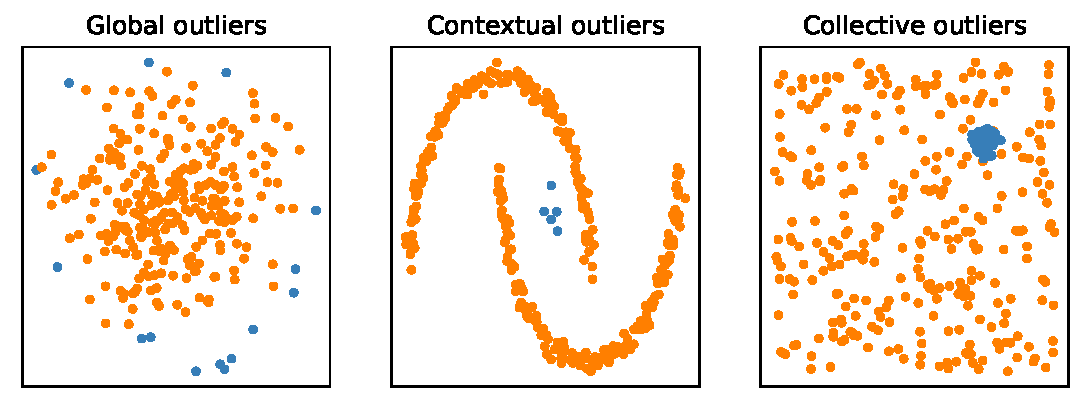
\includegraphics[width=0.7\textwidth]{../imgs/outlier_examples.pdf}
        \caption{Types of outliers}
    \end{figure}

    \begin{itemize}
        \item \textbf{Fig 1a:} Global outliers
        \item \textbf{Fig 1b:} Contextual outliers -- Given the dataset has two clusters, each one has a moon shape.
        \item \textbf{Fig 1c:} Blue points are collective outliers because the density of those points is much higher than the rest.
    \end{itemize}

\end{frame}

%-------------------------------------------------------------------------------
\begin{frame}
    \frametitle{2020 361 Exam Question 4 -- Outlier / Anomaly Detection}
    \small

    The following figure shows the monthly telecom usage activity in a specific area across
    several years. You were tasked to identify whether outliers exist in the data.

    \begin{figure}
        \centering
        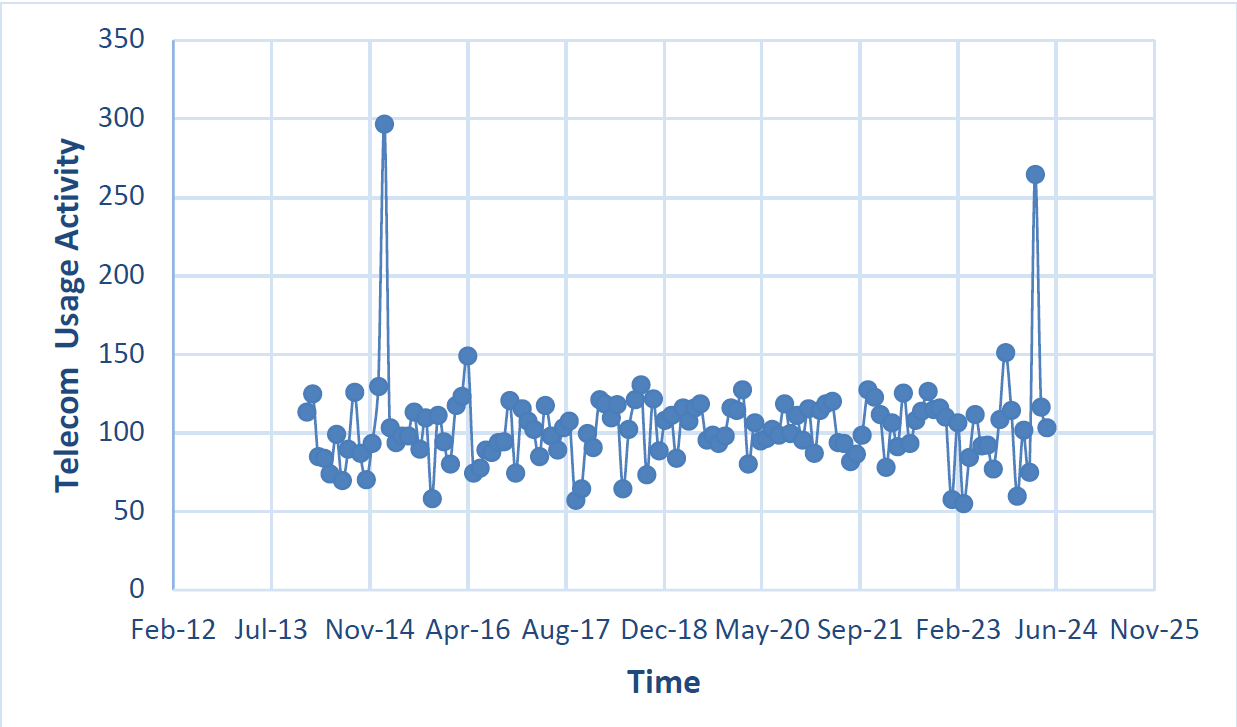
\includegraphics[width=0.6\textwidth]{../imgs/question4.png}
        % \caption{Monthly telecom usage}
    \end{figure}
    
    What outlier detection technique would you use to identify whether outliers exist for this case?
\end{frame}

%-------------------------------------------------------------------------------
\begin{frame}
    \frametitle{2020 361 Exam Question 4 -- Outlier / Anomaly Detection}

    \begin{columns}[]
        \begin{column}{0.5\textwidth}
            \begin{figure}
                \centering
                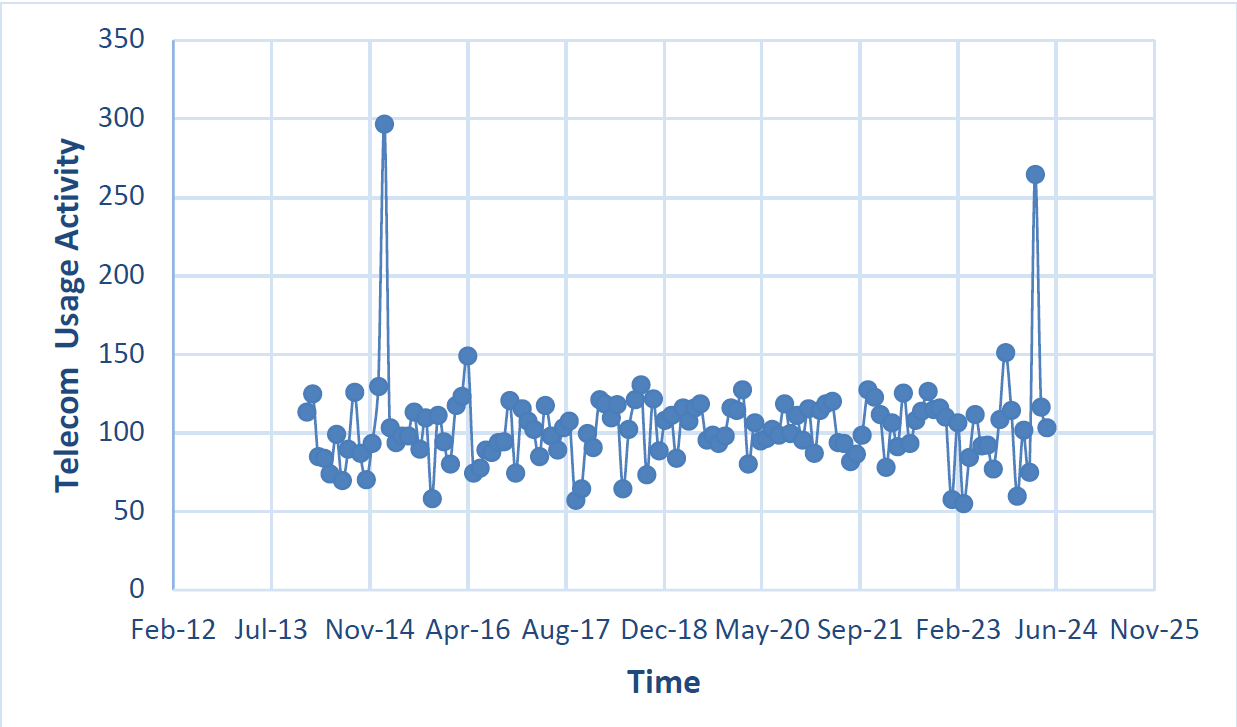
\includegraphics[width=\textwidth]{../imgs/question4.png}
                % \caption{Monthly telecom usage}
            \end{figure}
        \end{column}
        \begin{column}{0.5\textwidth}
            \begin{itemize}
                \item No obvious periodic pattern;
                \item No dramatic density changes;
                \item Unlikely to have contextual outlier and collective outlier;
                \item We apply the \textbf{statistical approach -- parametric method} to find global outliers.
                \item There are multiple ways to solve this problem.
            \end{itemize}
        \end{column}
    \end{columns}
    
\end{frame}

%-------------------------------------------------------------------------------
\begin{frame}
    \frametitle{2020 361 Exam Question 4 -- Outlier / Anomaly Detection}
    
    \begin{columns}[]
        \begin{column}{0.5\textwidth}
            \begin{figure}
                \centering
                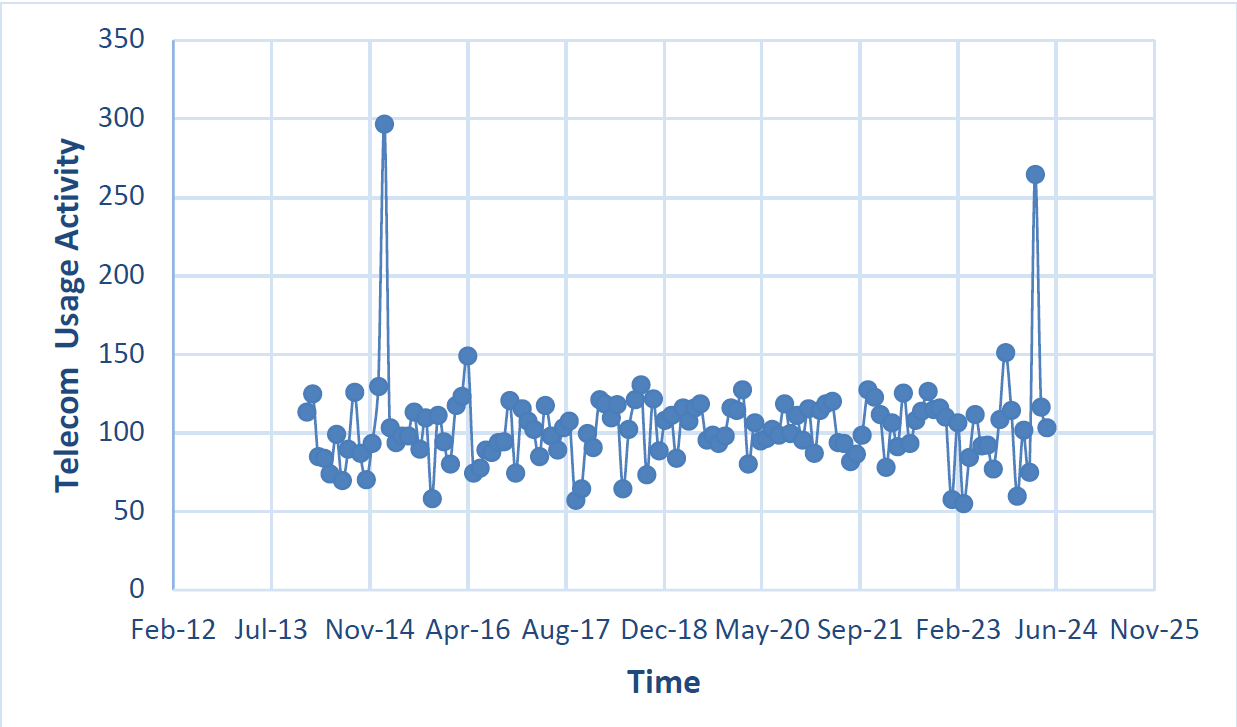
\includegraphics[width=\textwidth]{../imgs/question4.png}
                % \caption{Monthly telecom usage}
            \end{figure}
        \end{column}
        \begin{column}{0.5\textwidth}
            \begin{itemize}
                \item \textbf{Parametric method:} Assume the samples are drawn from a normal distribution, estimate the maximum likelihood of mean $\mu$ and standard deviation $\sigma$.
                \item We know that the $\mu \pm 3 \sigma$ region contains $99.7\%$. According to z-score, if $z=\frac{|x_i-\bar{x}|}{s} > 3$, the sample $x_i$ is generated by the normal distribution is less than $\frac{0.3}{2}=0.15\%$.
                \item Note that we do not know the population mean and standard deviation, we only have sample mean and sample standard deviation.
            \end{itemize}
        \end{column}
    \end{columns}

\end{frame}

%-------------------------------------------------------------------------------
\begin{frame}
    \frametitle{2020 361 Exam Question 4 -- Outlier / Anomaly Detection}
    
    \begin{columns}[]
        \begin{column}{0.5\textwidth}
            \begin{figure}
                \centering
                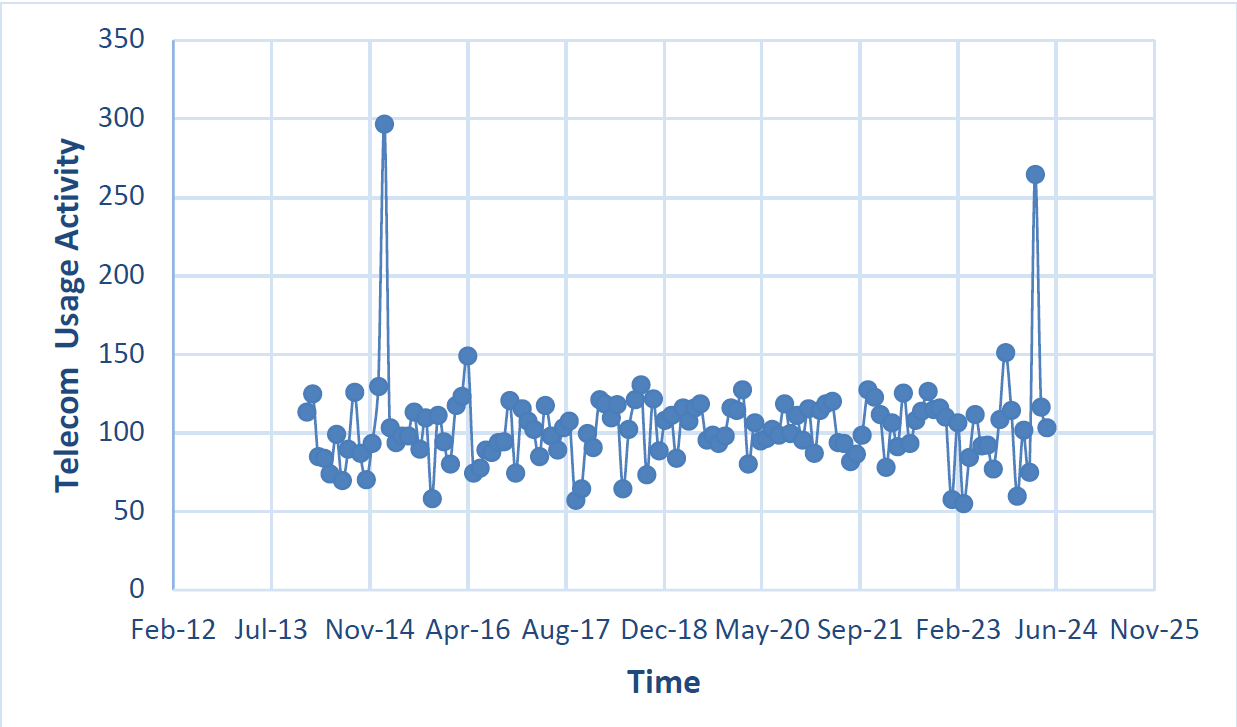
\includegraphics[width=\textwidth]{../imgs/question4.png}
                % \caption{Monthly telecom usage}
            \end{figure}
        \end{column}
        \begin{column}{0.5\textwidth}
            \begin{itemize}
                \item Based on observation, each grid contains around 14 points, we have 110 data points in total. 
                \item $\bar{x} = \frac{1}{N}\sum^N_{i=1}x_i \approx 100$
                \item $s = \sqrt{\frac{1}{N-1}\sum^N_{i=1}(x_i - \bar{x})^2} \approx 20$
                \item $\frac{|300 - 100|}{20}=10 > 3$, an outlier
                \item $\frac{|270 - 100|}{20}=8.5 > 3$, an outlier
                \item $\frac{|150 - 100|}{20}=2.5 < 3$, not an outlier
                \item $\frac{|55 - 100|}{20}=2.25 < 3$, not an outlier
            \end{itemize}
        \end{column}
    \end{columns}

\end{frame}

%-------------------------------------------------------------------------------
\begin{frame}
    \frametitle{Tutorial Question 1 -- Anomaly Detection}
    
    \begin{block}{Question 1}
        You are given the following list of 2D data points. 
        [[1; 1]; [1; 2]; [2; 2]; [2; 1]; [3; 3]; [2; 5]; [2; 3]] If you had to select one point to be anomalous, 
        which would you pick? Explain your answer. Please link your explanation to an anomaly detection technique.
    \end{block}



    There are multiple ways to solve this problem.\\
    Let's use \textbf{distance-based outlier detection}.


\end{frame}

%-------------------------------------------------------------------------------
\begin{frame}[t]
    \frametitle{Tutorial Question 1 -- Anomaly Detection}
    \small
    
    \begin{columns}[t]
        \begin{column}{0.5\textwidth}
            \textbf{Distance-based outlier detection}

            \begin{table}[]
                \scriptsize
                \begin{tabular}{c|ccccccc}
                             & \textbf{1,1} & \textbf{1,2} & \textbf{2,2} & \textbf{2,1} & \textbf{3,3} & \textbf{2,5} & \textbf{2,3} \\ \hline
                \textbf{1,1} & 0            & 1            & 2            & 1            & 4            & 5            & 3            \\
                \textbf{1,2} & 1            & 0            & 1            & 2            & 3            & 4            & 2            \\
                \textbf{2,2} & 2            & 1            & 0            & 1            & 2            & 3            & 1            \\
                \textbf{2,1} & 1            & 2            & 1            & 0            & 3            & 4            & 2            \\
                \textbf{3,3} & 4            & 3            & 2            & 3            & 0            & 3            & 1            \\
                \textbf{2,5} & 5            & 4            & 3            & 4            & 3            & 0            & 2            \\
                \textbf{2,3} & 3            & 2            & 1            & 2            & 1            & 2            & 0           
                \end{tabular}
                \caption{Manhattan Distance Matrix}
            \end{table}

            \[
                \frac{|\{o' | \text{dist}(o, o') \le r\}|}{|D|} \le \pi
            \]
            where $|D|$ is the {\em cardinality} of the set $D$.\\
            \hspace*{1em}

            We need to define the hyperparameters: $r$ and $\pi$.
        \end{column}
        \begin{column}{0.5\textwidth}
            The number of data points, $|D|$, is 7.\\
            Let $r=2$,

            \begin{table}[]
                \scriptsize
                \begin{tabular}{c|c|c}
                             &  \textbf{\# of objects within $r$} & \textbf{Divide by $|D|$}\\ \hline
                \textbf{1,1} &  3 & 0.43 \\
                \textbf{1,2} &  4 & 0.57 \\
                \textbf{2,2} &  5 & 0.71 \\
                \textbf{2,1} &  4 & 0.57 \\
                \textbf{3,3} &  2 & 0.29 \\
                \rowcolor[HTML]{34CDF9}\textbf{2,5} &  1 & 0.14 \\
                \textbf{2,3} &  5 & 0.71   
                \end{tabular}
                \caption{The \# of neighbours within $r$}
            \end{table}

            If we select only one point as an outlier, we can set $\pi$ to any value between $0.14$ and $0.29$, e.g. $0.15$.\\
            Therefore, we identify $[2;5]$ is an outlier.\\            
        \end{column}
    \end{columns}
\end{frame}


%-------------------------------------------------------------------------------
\begin{frame}
    \frametitle{Tutorial Question 2 -- Density-based Approach: Local Outlier Factor (LOF)}
    \footnotesize

    \begin{block}{Question 2}
        Consider a set of points (0,0), (1,0), (0,1), (3,0). 
        Calculate the LOF score for the points using Manhattan distance and $k$ is 2.
    \end{block}
    
    \begin{columns}[t]
        \begin{column}{0.5\textwidth}

            \begin{figure}
                \centering
                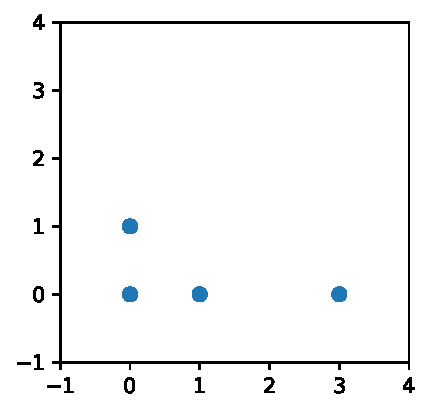
\includegraphics[width=0.35\textwidth]{../imgs/outlier_lof.pdf}
            \end{figure}

            \begin{table}[]
                \scriptsize
                \begin{tabular}{c|cccc}
                             & \textbf{a (0,0)} & \textbf{b (1,0)} & \textbf{c (0,1)} & \textbf{d (3,0)} \\ \hline
                \textbf{a (0,0)} & 0            & 1            & 1            & 3            \\
                \textbf{b (1,0)} & 1            & 0            & 2            & 2            \\
                \textbf{c (0,1)} & 1            & 2            & 0            & 4            \\
                \textbf{d (3,0)} & 3            & 2            & 4            & 0           
                \end{tabular}
                \caption{Manhattan distance matrix}
            \end{table}
        \end{column}
        \begin{column}{0.5\textwidth}
            \begin{table}[]
                \scriptsize
                \begin{tabular}{c|cc}
                             & $\text{dist}_2(o)$ & $N_2(o)$ \\ \hline
                \textbf{a (0,0)} & 1 & 2 \\
                \textbf{b (1,0)} & 2 & \textcolor{blue}{3} \\
                \textbf{c (0,1)} & 2 & 2 \\
                \textbf{d (3,0)} & 3 & 2  
                \end{tabular}
                \caption{Distance between data point $o$ and its k-th nearest neighbour ($k=2$)}
            \end{table}
            We denote the set of $k$-nearest neighbours as $N_k(o)$:
            \[
                N_k(o) = \{o' | o' \in D, \text{dist}(o, o') \le \text{dist}_k(o)\}
            \]
            \textbf{Note:} $|N_k(o)|$ may contain more than $k$ objects, because objects may have same distance.
        \end{column}
    \end{columns}

\end{frame}

%-------------------------------------------------------------------------------
\begin{frame}
    \frametitle{Tutorial Question 2 -- LOF}

    Let $o'$ be a neighbour of $o$, to avoid $\text{dist}(o, o')$ is too small, we compute the reachability distance from $o$ to $o'$:
    \[
        \text{reachdist}_k(o' \leftarrow o) = \max\{\text{dist}_k(o), \text{dist}(o, o')\}
    \]
    
    Note that reachability distance is not symmetric, thus 
    \[
        \text{reachdist}_k(o \leftarrow o') \neq \text{reachdist}_k(o' \leftarrow o)
    \]

    \begin{figure}
        \centering
        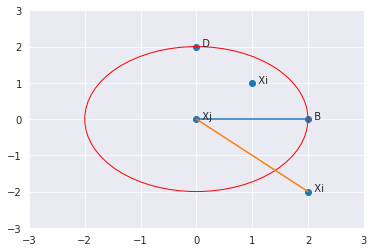
\includegraphics[width=0.4\textwidth]{../imgs/reachdist.png}
    \end{figure}

\end{frame}

%-------------------------------------------------------------------------------
\begin{frame}[t]
    \frametitle{Tutorial Question 2 -- LOF}
    \small

    \begin{equation*}
        \begin{array}{rlll}
            \rowcolor[HTML]{34CDF9} \text{reachdist}_2(b \leftarrow a) & = \max\{\text{dist}_2(a), \text{dist}(a, b)\} & = \max\{1, 1\} & = 1\\
            \text{reachdist}_2(c \leftarrow a) & = \max\{\text{dist}_2(a), \text{dist}(a, c)\} & = \max\{1, 1\} & = 1\\
            \text{reachdist}_2(d \leftarrow a) & = \max\{\text{dist}_2(a), \text{dist}(a, d)\} & = \max\{1, 3\} & = 3\\
            \rowcolor[HTML]{34CDF9} \text{reachdist}_2(a \leftarrow b) & = \max\{\text{dist}_2(b), \text{dist}(b, a)\} & = \max\{2, 1\} & = 2\\
            \text{reachdist}_2(c \leftarrow b) & = \max\{\text{dist}_2(b), \text{dist}(b, c)\} & = \max\{2, 2\} & = 2\\
            \text{reachdist}_2(d \leftarrow b) & = \max\{\text{dist}_2(b), \text{dist}(b, d)\} & = \max\{2, 2\} & = 2\\
            \text{reachdist}_2(a \leftarrow c) & = \max\{\text{dist}_2(c), \text{dist}(c, a)\} & = \max\{2, 1\} & = 2\\
            \text{reachdist}_2(b \leftarrow c) & = \max\{\text{dist}_2(c), \text{dist}(c, b)\} & = \max\{2, 2\} & = 2\\
            \text{reachdist}_2(d \leftarrow c) & = \max\{\text{dist}_2(c), \text{dist}(c, d)\} & = \max\{2, 4\} & = 4\\
            \text{reachdist}_2(a \leftarrow d) & = \max\{\text{dist}_2(d), \text{dist}(d, a)\} & = \max\{3, 3\} & = 3\\
            \text{reachdist}_2(b \leftarrow d) & = \max\{\text{dist}_2(d), \text{dist}(d, b)\} & = \max\{3, 2\} & = 3\\
            \text{reachdist}_2(c \leftarrow d) & = \max\{\text{dist}_2(d), \text{dist}(d, c)\} & = \max\{3, 4\} & = 4\\
        \end{array}
    \end{equation*}

    \[
        \text{reachdist}_k(o \leftarrow o') \neq \text{reachdist}_k(o' \leftarrow o)
    \]
\end{frame}

%-------------------------------------------------------------------------------
\begin{frame}[t]
    \frametitle{Tutorial Question 2 -- LOF}
    
    The {\em Local Reachability Density} (LRD) of an object $o$ is defined as
    \[
        \text{lrd}_k(o) = \frac{|N_k(o)|}{\sum_{o' \in N_k(o)} \text{reachdist}_k(o \leftarrow o')}
        \]
        
    \begin{equation*}
        \footnotesize
        \begin{array}{rlll}
            \text{lrd}_2(a) & = |N_2(a)| / (\text{reachdist}_2(a \leftarrow b) + \text{reachdist}_2(a \leftarrow c))                                      & = 2 / (2 + 2) & = 0.5\\
            \text{lrd}_2(b) & = |N_2(b)| / (\text{reachdist}_2(b \leftarrow a) + \text{reachdist}_2(b \leftarrow c) + \text{reachdist}_2(b \leftarrow d)) & = 3 / (1+2+3) & = 0.5\\
            \text{lrd}_2(c) & = |N_2(c)| / (\text{reachdist}_2(c \leftarrow a) + \text{reachdist}_2(c \leftarrow b))                                      & = 2 / (1 + 2) & = 0.667\\
            \text{lrd}_2(d) & = |N_2(d)| / (\text{reachdist}_2(d \leftarrow a) + \text{reachdist}_2(d \leftarrow b))                                      & = 2 / (3 + 2) & = 0.4\\
        \end{array}
    \end{equation*}

\end{frame}

%-------------------------------------------------------------------------------
\begin{frame}[t]
    \frametitle{Tutorial Question 2 -- LOF}
    
    The {\em Local Outlier Factor} (LOF) of an object $o$ is
    \[
        \text{LOF}_k(o) = \frac{\sum_{o' \in N_k(o)} \frac{\text{lrd}_k(o')}{\text{lrd}_k(o)}}{|N_k(o)|} 
        = \frac{\sum_{o' \in N_k(o)} \text{lrd}_k(o')}{|N_k(o)| \cdot \text{lrd}_k(o)}
    \]
        
    \begin{equation*}
        \footnotesize
        \begin{array}{rlll}
            \text{LOF}_2(a) & = (\text{lrd}_2(b) + \text{lrd}_2(c)) / (|N_2(a)| \cdot \text{lrd}_2(a)) & = (0.5+0.667) / (2\times 0.5)& = 1.167\\
            \text{LOF}_2(b) & = (\text{lrd}_2(a) + \text{lrd}_2(c) + \text{lrd}_2(d)) / (|N_2(b)| \cdot \text{lrd}_2(b))  & = (0.5+0.667+0.4) / (3\times 0.5)& \approx 1.045\\
            \text{LOF}_2(c) & = (\text{lrd}_2(a) + \text{lrd}_2(b)) / (|N_2(c)| \cdot \text{lrd}_2(c))  & = (0.5+0.5) / (2\times 0.667)& \approx 0.750\\
            \text{LOF}_2(d) & = (\text{lrd}_2(a) + \text{lrd}_2(b)) / (|N_2(d)| \cdot \text{lrd}_2(d))  & = (0.5+0.5) / (2\times 0.4)& = 1.25\\
        \end{array}
    \end{equation*}

\end{frame}

%-------------------------------------------------------------------------------
\begin{frame}
    \frametitle{Tutorial Question 2 -- LOF}
    
    \begin{figure}
        \centering
        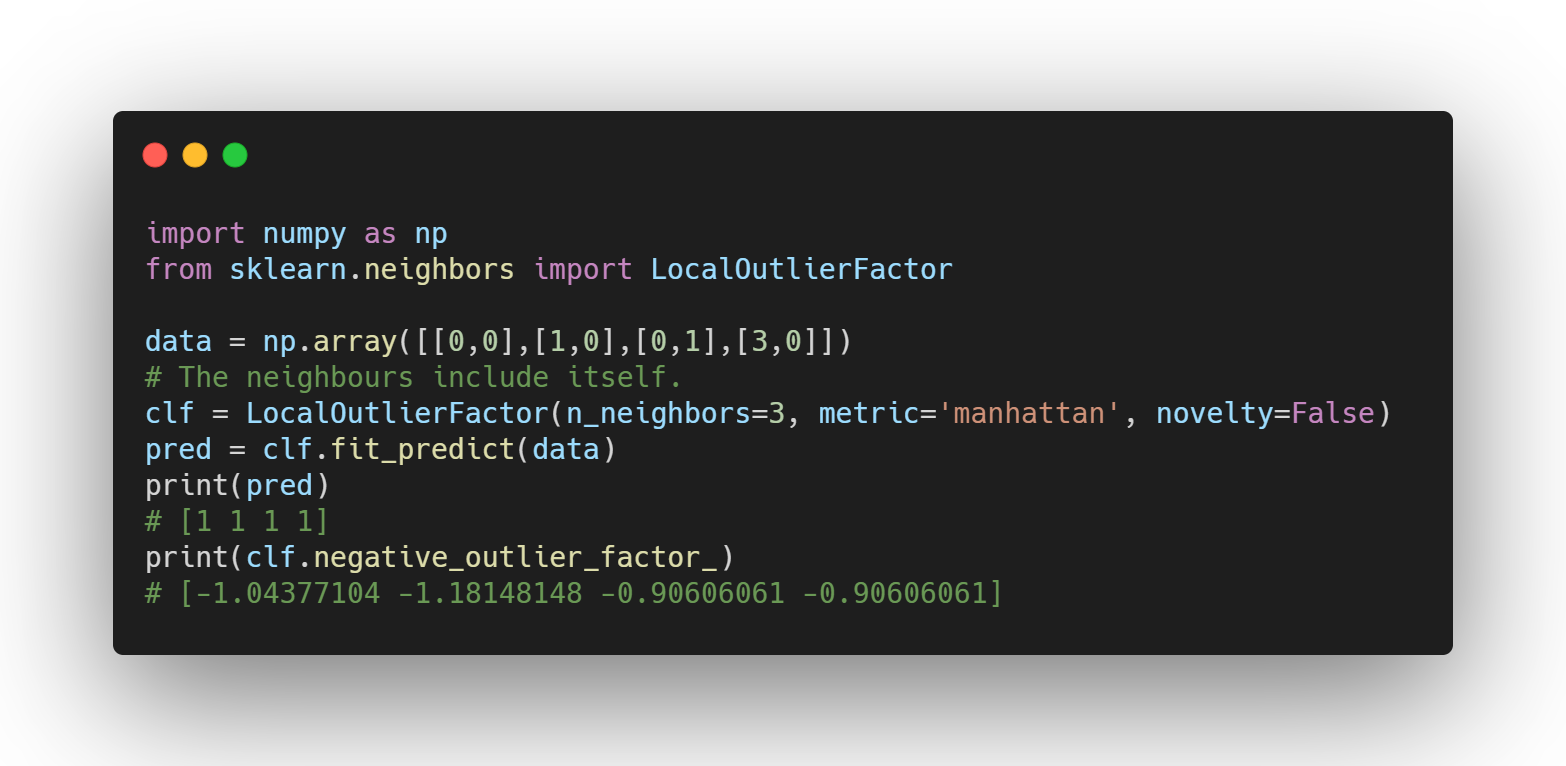
\includegraphics[width=\textwidth]{../imgs/question2_lof_code.png}
    \end{figure}
\end{frame}

%-------------------------------------------------------------------------------
\begin{frame}
    \frametitle{Tutorial Question 3 -- Supervised}
    \footnotesize 

    \begin{block}{Question 3}
        What is a difference, between a supervised, semi-supervised, and unsupervised anomaly detection techniques?
    \end{block}

    \textbf{Supervised}
    \begin{itemize}
        \item With labels, i.e., normal objects vs. outliers
        \item Binary classification problem
        \item Extremely imbalanced, majority of the objects are normal.
    \end{itemize}

    \textbf{Unsupervised}
    \begin{itemize}
        \item Labels are not available
        \item Clustering based methods
    \end{itemize}

    \textbf{Semi-supervised}
    \begin{itemize}
        \item Some labeled examples is feasible, the number of such labeled examples is small.
        \item Combining classification-based and clustering based methods
        \item Use the one-class model to label normal objects, e.g. One-class SVM
    \end{itemize}
\end{frame}

%-------------------------------------------------------------------------------
\section{Data Stream Mining}
\begin{frame}
    \frametitle{Tutorial Question 6 -- Data Stream}
    
    \begin{block}{Question 6}
        Give examples of three requirements for data stream mining that makes it different from regular data mining.
    \end{block}

    Examples:
    \begin{itemize}
        \item Web data, e.g. Amazon web orders, video steaming (real-time decoding)
        \item IoT sensors, e.g. Real-time temperature monitoring, blood pressure monitors, step monitor on a smartwatch
        \item Finance, e.g. Real-time stock price data
        \item Transportation and supply-chain, e.g. traffic information, pack-house logistic
    \end{itemize}

    Requirements:
    \begin{itemize}
        \item Process one instance at a time, and only inspect it once
        \item Time and space constraint
        \item Need to adapt changes (Concept drift)
    \end{itemize}
\end{frame}

%-------------------------------------------------------------------------------
\begin{frame}
    \frametitle{Tutorial Question 3 -- Sliding Window}
    
    \begin{block}{Question 3}
        When would you use a sliding window technique as compared to a reservoir sampling technique.
    \end{block}

    \textbf{Reservoir Sampling}
    \begin{itemize}
        \item A randomized algorithm for choosing a {\em simple random sample} without
        replacement of $k$ items from a population of unknown size in a single
        pass over the items.
        \item No matter how many stream elements $t$ have been read
        so far, each of them is currently in the reservoir with the same
        probability, $k/t$.
        \item Maintains a fixed-size uniform random sample
    \end{itemize}
\end{frame}

%-------------------------------------------------------------------------------
\begin{frame}
    \frametitle{Tutorial Question 3 -- Sliding Window}
    
    \begin{block}{Question 3}
        When would you use a sliding window technique as compared to a reservoir sampling technique.
    \end{block}

    \textbf{Sliding Window}
    \begin{itemize}
        \item Only  consider the last $n$ samples
        \item Clear way to bound memory
        \item Natural in applications: Emphasizes the most recent data
        \item Do not keep the old samples outside the current window
    \end{itemize}
\end{frame}

%-------------------------------------------------------------------------------
\begin{frame}
    \frametitle{Concept Drift}
    \begin{example}
        You use a real-time temperature sensor to predict the weather in Wellington.
        The model is trained from the data which are gathered from Wellington. The model shows high performance, 
        but there is a dramatic performance drop when using it to predict the weather in New York.
    \end{example}

    \begin{itemize}
        \item \textbf{Concept Drift} describes a change in the distribution of input data and labels over time.
        \item It may cause prediction accuracy to deteriorate over time.
    \end{itemize}
    
    Types of concept drift:
    \begin{itemize}
        \item \textbf{Real} concept drift: The relationship between the input data and label has changed. e.g. The concept of the keyword -- "Doge" on Twitter.
        \item \textbf{Virtual} concept drift: The distribution of input data has changed, but not the decision boundary. e.g. School holidays, less sales from the food court, the distribution changes, but the purchase pattern still holds.
    \end{itemize}
\end{frame}

%-------------------------------------------------------------------------------
\begin{frame}
    \frametitle{Drift Detection Method (DDM)}
    
    \begin{itemize}
        \item DDM monitors the number of errors produces by a model learned on the previous stream items.
        \item Let $P_t$ denote the error rate of the predictor at time $t$. 
        Given the number of errors in a sample of $t$ examples, its standard deviation at time t is given by:
        \[
            S_t = \sqrt{P_t(1-P_t)/t}
        \]
        \item DDM stores the smallest value of the error rates $P_{\text{min}}$ observed up to time $t$, and the standard deviation $S_{\text{min}}$ at that point.
        \item \textbf{Warning:} If $P_t + S_t \geq P_{\text{min}} + 2 S_{\text{min}}$, \textbf{new samples} are stored in anticipation of a possible change.
        \item \textbf{Change:} If $P_t + S_t  \geq P_{\text{min}} + 3 S_{\text{min}}$, a \textbf{new model} is built using the examples stored since the warning. Reset $P_{\text{min}}$ and $S_{\text{min}}$.
    \end{itemize}
\end{frame}

%-------------------------------------------------------------------------------
\begin{frame}[t]
    \frametitle{Tutorial Question 1 -- Drift Detection Method (DDM)}

    \begin{block}{Question 1}
        DDM has the drawback that it may take a long time to react to changes after a long period without change.
        Suggest a couple of ways to fix this, possibly at the cost of introducing some parameters.
    \end{block}
    
    \begin{itemize}
        \item DDM has difficulties when the change is \textbf{slowly} gradual. 
        \item  The examples will be stored for long time, the drift level can take too much time to trigger and the examples memory can be exceeded.
        \item {\em Early Drift Detection Method} (EDDM) by Baena-Garcıa, et al. (2006). The idea is to keep track of the \textbf{average distance between two errors} instead of only the error rate.
        It assumes that the distance between two occurrences of classification errors increases as a stable concept is being learnt.
    \end{itemize}
\end{frame}

% %-------------------------------------------------------------------------------
% \begin{frame}
%     \frametitle{Adaptive sliding window (ADWIN)}
    
%     \begin{itemize}
%         \item ADWIN keeps a variable-length window of recently seen items.
%     \end{itemize}
    
% \end{frame}

% %-------------------------------------------------------------------------------
% \begin{frame}
%     \frametitle{}
    
%     \begin{block}{Question 2}
%         Consider the implementation of ADWIN with the Hoeffding-based test. Discuss how ADWIN will react to:
% (1) A stream with an abrupt change. After a long stream of bits with average 0, at some time T the average
% suddenly changes to 1 6= 0.
% (2) Gradual after a long stream of bits with average 0, at time T the average starts increasing linearly so that
% the average at time t > T is t+1 = t + , with  a small value.
%     \end{block}
% \end{frame}

\end{document}


